\documentclass[11pt]{article}
\usepackage[margin=20mm]{geometry}
\usepackage{amsmath}
\usepackage{float}
\usepackage{subfig}
\usepackage{listings,color,enumitem}
\definecolor{mygreen}{RGB}{28,172,0} % color values Red, Green, Blue
\definecolor{mylilas}{RGB}{170,55,241}
\usepackage{graphicx}

%\graphicspath{results/}
\title{Homework 3\\ \vspace{2mm}\Large{16-720A Computer Vision }}
\author{Matthew Swenson}

\begin{document}
	\maketitle
	
\section*{Q 1.3}
\begin{figure}[H]
\centering
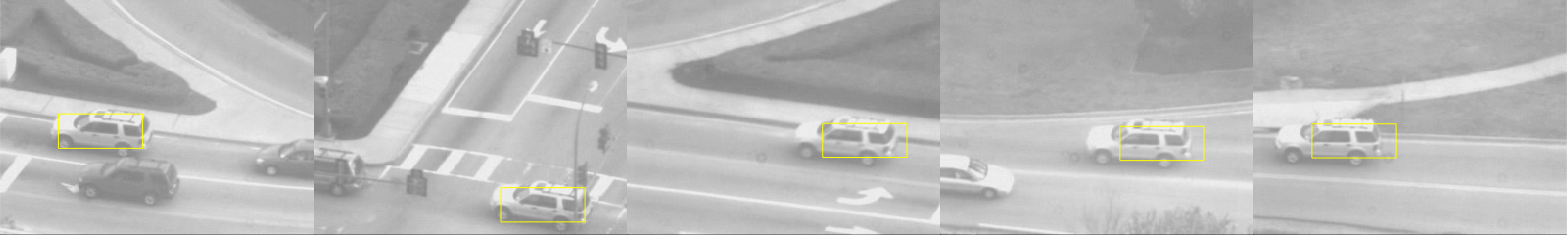
\includegraphics[width=\textwidth]{cartest.png}
\caption{Basic Lucas-Kanade template tracking.}
\end{figure}
\section*{Q 1.4}
\begin{figure}[H]
\centering
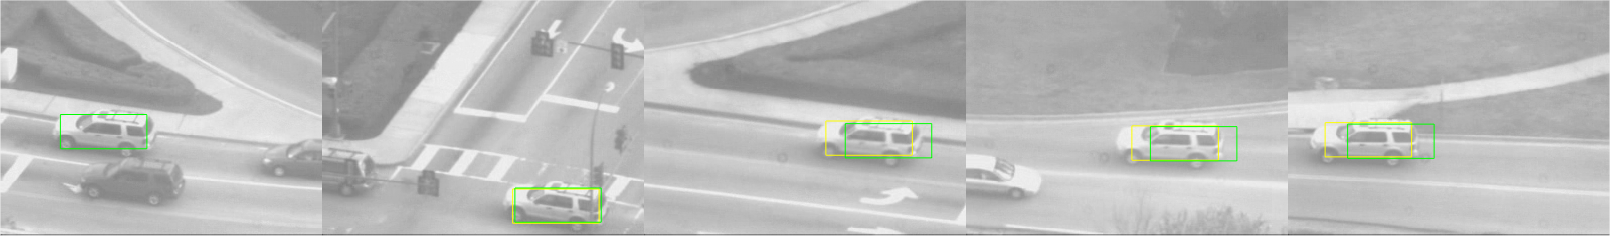
\includegraphics[width=\textwidth]{cartestcorrected.png}
\caption{Lucas-Kanade template tracking with drift correction. The green boxes are the original Lucas-Kanade
algorithm, the yellow boxes are the drift corrected version.}
\end{figure}
\section*{Q 2.1}
Given
$$
\mathcal{I}_{t+1}(\mathbf{x}) =\mathcal{I}_t(\mathbf{x}) +\sum_{k=1}^{K} w_k\mathcal{B}_{k
}(\mathbf{x}) 
$$
we can find $\mathbf{w}$:
$$
    %w = \left(\mathcal{I}_{t+1}(\mathbf{x}) - \mathcal{I}_t(\mathbf{x}) \right) \[\]^{-1}
    w = \left(\mathcal{I}_{t+1}(\mathbf{x}) - \mathcal{I}_t(\mathbf{x}) \right) \left[\{\mathcal{B}_k\}_{k=1}^K\right]^{-1}
$$
\begin{figure}[H]
\centering
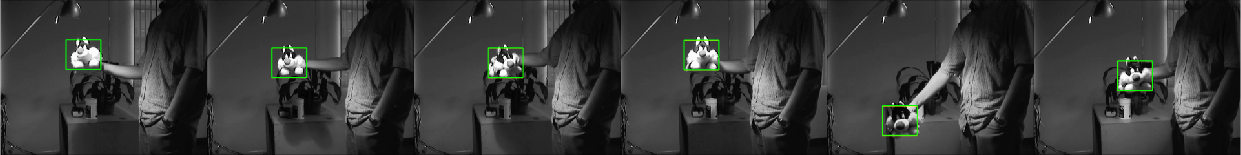
\includegraphics[width=\textwidth]{sylvtest.png}
\caption{Appearance basis tracking to more accurately track a template of Sylvester the cat. Yellow is the original Lucas-Kanade algorithm, 
        green is the basis-corrected Lucas-Kanade algorithm. The basic algorithm performs well enough that there is little observable difference
    in this basic test.}
\end{figure}

\section*{Q 3.3}
\begin{figure}[H]
\centering
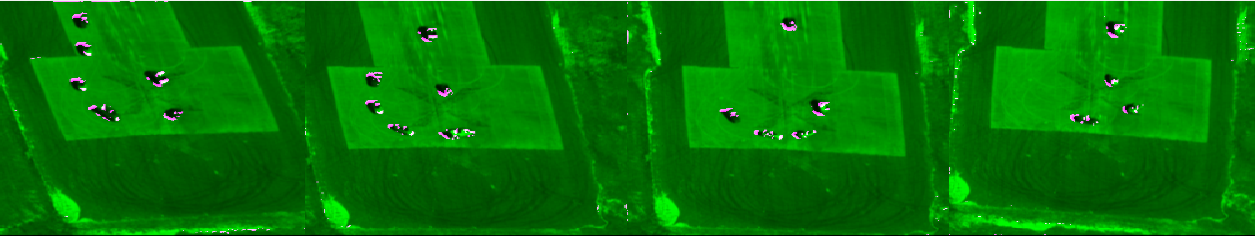
\includegraphics[width=\textwidth]{aerialtest.png}
\caption{Dominant affine motion removal with Lucas-Kanade. The pink dots are what is actually moving in the ground plane.}
\end{figure}

\end{document}
